\section{monasca-log-api - REST'owe API dla logów}
\label{chapter:monasca:monasca_log_api}

\textbf{monasca-log-api} jest to \textbf{REST}-owe API skonstruowane jako
brama wejściowa do odbierania logów od agentów (instancje \textbf{monasca-log-agent}
\ref{chapter:monasca:monasca_log_agent}).
    
    \subsection{Proces przysyłania danych}
    \begin{figure}[H]
        \centering
        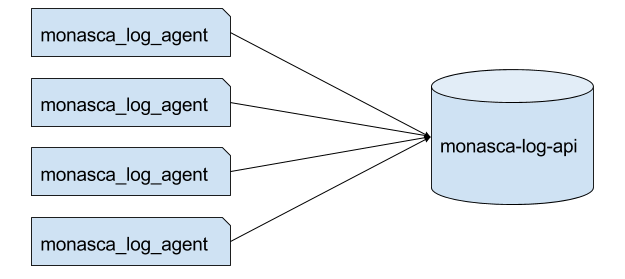
\includegraphics[width=0.80\textwidth]{images/monasca_log_api_data_flow}
        \caption[Relacja monasca-log-agent z monasca-log-api]{
            Relacja monasca-log-agent z monasca-log-api, źródło: opracowanie własne
        }
        \label{chapter:monasca:monasca_log_api:data_flow}
    \end{figure}
    Przesył danych inicjowany jest po stronie agenta. To, co zostanie przesłane
    do \textbf{monasca-log-api}, zależy w dużej mierze od konfiguracji agenta 
    \ref{chapter:monasca:monasca_log_agent:configuration}. Oprócz faktycznego
    logu, agent dodaje najczęściej informacje pozwalające na ustalenie jego pochodzenia (ścieżki, aplikacji) oraz
    datę pobrania rekordu. Po skompletowaniu wszystkich informacji wiadomość podlega
    transformacji do żądania HTTP i zostaje wysłana do serwera.
    
    \subsubsection{Struktura żądania}
    \begin{figure}[h]
        \centering
        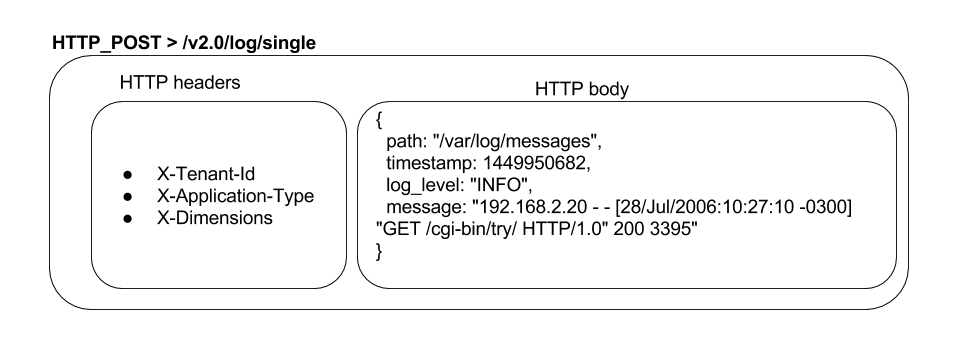
\includegraphics[width=0.80\textwidth]{images/monasca_log_api_request}
        \caption[Żądanie HTTP w monasca-log-api]{
             Żądanie HTTP w monasca-log-api, źródło: opracowanie własne
        }
        \label{chapter:monasca:monasca_log_api:request}
    \end{figure}
    Rysunek \ref{chapter:monasca:monasca_log_api:request} przedstawia przykładowe
    żądanie jakie agent może wysłać do serwera w postaci minimalnie wymaganej
    i akceptowanej przez aplikację. Dają się tu wyróżnić następujące nagłówki żądania:
    \begin{itemize}
        \item \textbf{X-Tenant-Id} - UUID jednoznacznie identyfikujący tenanta w chmurze,
        \item \textbf{X-Application-Type} - wskazuje na typ aplikacji, z której zebrano logi,
        \item \textbf{X-Dimensions} - wszelkie dane opisujące żądanie (nazwa hosta, adres IP hosta itp).
    \end{itemize}
    Stanowią one rodzaj uzupełniania dla logu przesłanego w ciele żądania. Faktyczna ilość nagłówków wygląda 
    jednak inaczej. W wyniku weryfikacji wartości \textbf{X-Tenant-Id} do listy dołączane są:
    \begin{itemize}
        \item \textbf{X-Identity-Status} - określający status autentykacji,
        \item \textbf{X-Roles} - zestaw uprawnień powiązanych z tenantem.
    \end{itemize}
    
    Również ciało żądania może być dużo większe. Niemniej jest to najczęściej łańcuch tekstowy
    interpretowany jako \textbf{application/json}, który zawierać będzie pole \textbf{message},
    ostatni odczytany wpis z monitorowanego pliku. Na rozmiar żądania natomiast największy wpływ będzie mieć
    to jak duży był log (na poziomie obserwowanego zasobu). 
    
    Każdy z agentów wysyła kolejne rekordy z monitorowanych plików pojedynczo jako
    ciało żądania HTTP\footnote{Request body lub message body - dane, które klient wysyła do serwera}.
    Zawiera ono surowe dane odczytane przez agenta. \textbf{monasca-log-api} nie zajmuje się normalizacją lub weryfikacją tych danych. Głównym tego powodem jest fakt, że struktura logu na poziomie
    serwera WWW jest rzeczą nieznaną. Wynika to z ilości potencjalnych źródeł, które 
    mogą przesyłać do niego dane. Niemniej walidacja istnieje, ale odnosi się do:
    \begin{itemize}
        \item rozmiaru przesłanych danych (walidacja dwupoziomowa),
        \item nagłówków żądania, które muszę odpowiadać ustalonemu formatowi
    \end{itemize}\cite{monasca_log_api_spec}.
    
    \subsubsection{Proces walidacji}
    \label{chapter:monasca:monasca_log_api:validation}
    
    Serwer nie przetworzy każdego żądania. Jednym z kryterium odrzucenia i
    tym samym walidacji jest rozmiar przesłanych danych. Konieczność wykonania tego kroku 
    związana jest z elementem odbierającym dane od \textbf{monasca-log-api}, a dokładniej z medium
    którymi informacje są przesyłane. \textbf{Kafka} - kolejka danych - może, w domyślnej konfiguracji,
    przyjąć jednorazowo 1MB (megabajt) danych. \textbf{monasca-log-api} pro-aktywnie eliminuje zbyt duże
    wiadomości, których próba wysłania zakończyłaby się niepowodzeniem. Walidacja odbywa się na dwóch poziomach:
    \begin{itemize}
        \item[poziom 0] - weryfikowany jest rozmiar samego żądania HTTP. Pod uwagę brany jest nagłówek
        \textbf{Content-Length}, dający informację o ilości (w bajtach) wysłanych przez klienta danych.
        Przekroczenie maksymalnej wartości powoduje wygenerowanie przez serwer odpowiedzi 
        \textbf{HTTP 413 :: Request Entity Too Large}. Wspomniany nagłówek jest szczególnie istotny,
        ponieważ pozwala na określenie, czy żądanie można lub nie przetworzyć bez konieczności
        odczytania właściwych danych. Z tego też powodu jego brak również uznawany jest za błąd.
        W odpowiedzi do klienta serwer wygeneruje błąd \textbf{HTTP 411 - Length Required}.
        \item[poziom 1] - następuje tuż przed wysłaniem wiadomości do \textbf{Kafki}. Po wykonaniu wszystkich
        operacji związanych z odczytem żądania, dodaniem meta danych do logu rozmiar wiadomości może się
        znacząco zwiększyć. Możliwa jest sytuacja, w której początkowy rozmiar jest zbliżony do 
        wartości maksymalnej, ale jej nie przekracza. \textbf{monasca-log-api} nie reaguje na poziomie 0. Wiadomość wysyłana do \textbf{Kafki} składa się jednak z większej ilości elementów,
        więc dodawanie ich może spowodować przekroczenie wartości granicznej. W tym wypadku jest to sytuacja
        tożsama z wewnętrznym błędem serwera, w jej wyniku, klient otrzyma odpowiedź
        \textbf{HTTP 500 - Internal Server Error}.
    \end{itemize}
    
    Warto w tym miejscu zaznaczyć, że zmiany w konfiguracji Kafki, odnoszące się do zwiększania
    maksymalnego rozmiaru wiadomości, są również odzwierciedlane w \textbf{monasca-log-api}. 
    
    \subsection{Dostarczanie danych}
    \begin{figure}[H]
        \centering
        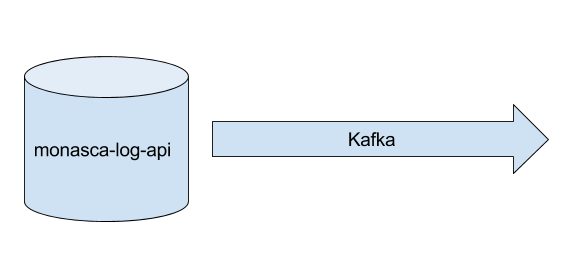
\includegraphics[width=0.80\textwidth]{images/monasca_log_api_to_kafka}
        \caption[monasca-log-api a Kafka]{
            monasca-log-api a Kafka, źródło: opracowanie własne
        }
        \label{chapter:monasca:monasca_log_api:kafka}
    \end{figure}
    Dane z \textbf{monasca-log-api} trafiają do kolejki \textbf{Kafka}.
    Dla każdej z wiadomości obliczana jest specjalna wartość - klucz. Pozwala on na określenie partycji
    wewnątrz Kafki. Dzięki temu dane dystrybuowane są równomiernie. Jest to konieczne z uwagi
    na wolumin danych, które muszą wejść do kolejki. Bez tej operacji mogłoby dojść do przepełnienia się
    bufora wewnątrz Kafki i wiadomości mogłyby zostać utracone. W przypadku logów o strategicznym
    znaczeniu dla chociażby analizowania przyczyn potencjalnych błędów, jest to sytuacja niedopuszczalna.
    